L'interface utilisateur a été implémenté à l'aide de la bibliothèque graphique Tkinter. Elle dispose de deux modules:
\begin{enumerate}
	\item un module d'édition du code jouet permettant le chargement, l'édition et l'enregistrement de scripts
	\item un module d'exécution disponible après compilation permettant:
	\begin{itemize}
		\item l'affichage du code assembleur et du binaire associé;
		\item le suivi des registres, mémoire et pointeurs associés;
		\item le suivi des appels UAL;
		\item une sortie et une entrée.
	\end{itemize}
\end{enumerate}
Les deux modules disposent par ailleurs d'un affichage permettant de commenter l'exécution en cours.

\begin{figure}[h!]
	\centering
	\begin{subfigure}{\textwidth}
		\centering
		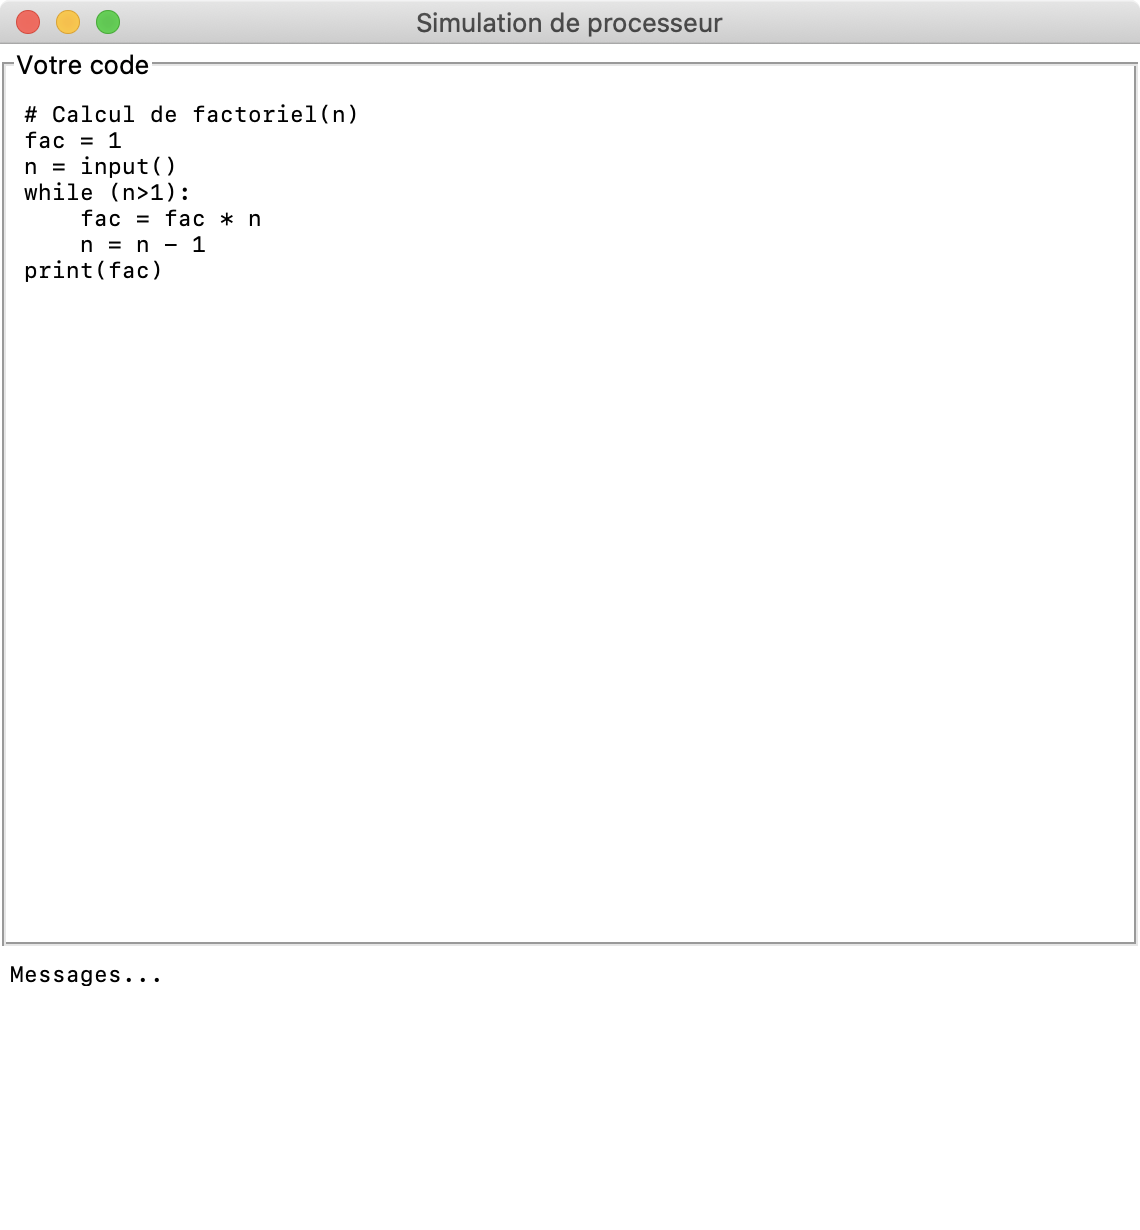
\includegraphics[height=8cm]{./Pictures/EditGUI.png}
		\caption{Module Édition}
	\end{subfigure}
	\begin{subfigure}{\textwidth}
		\centering
	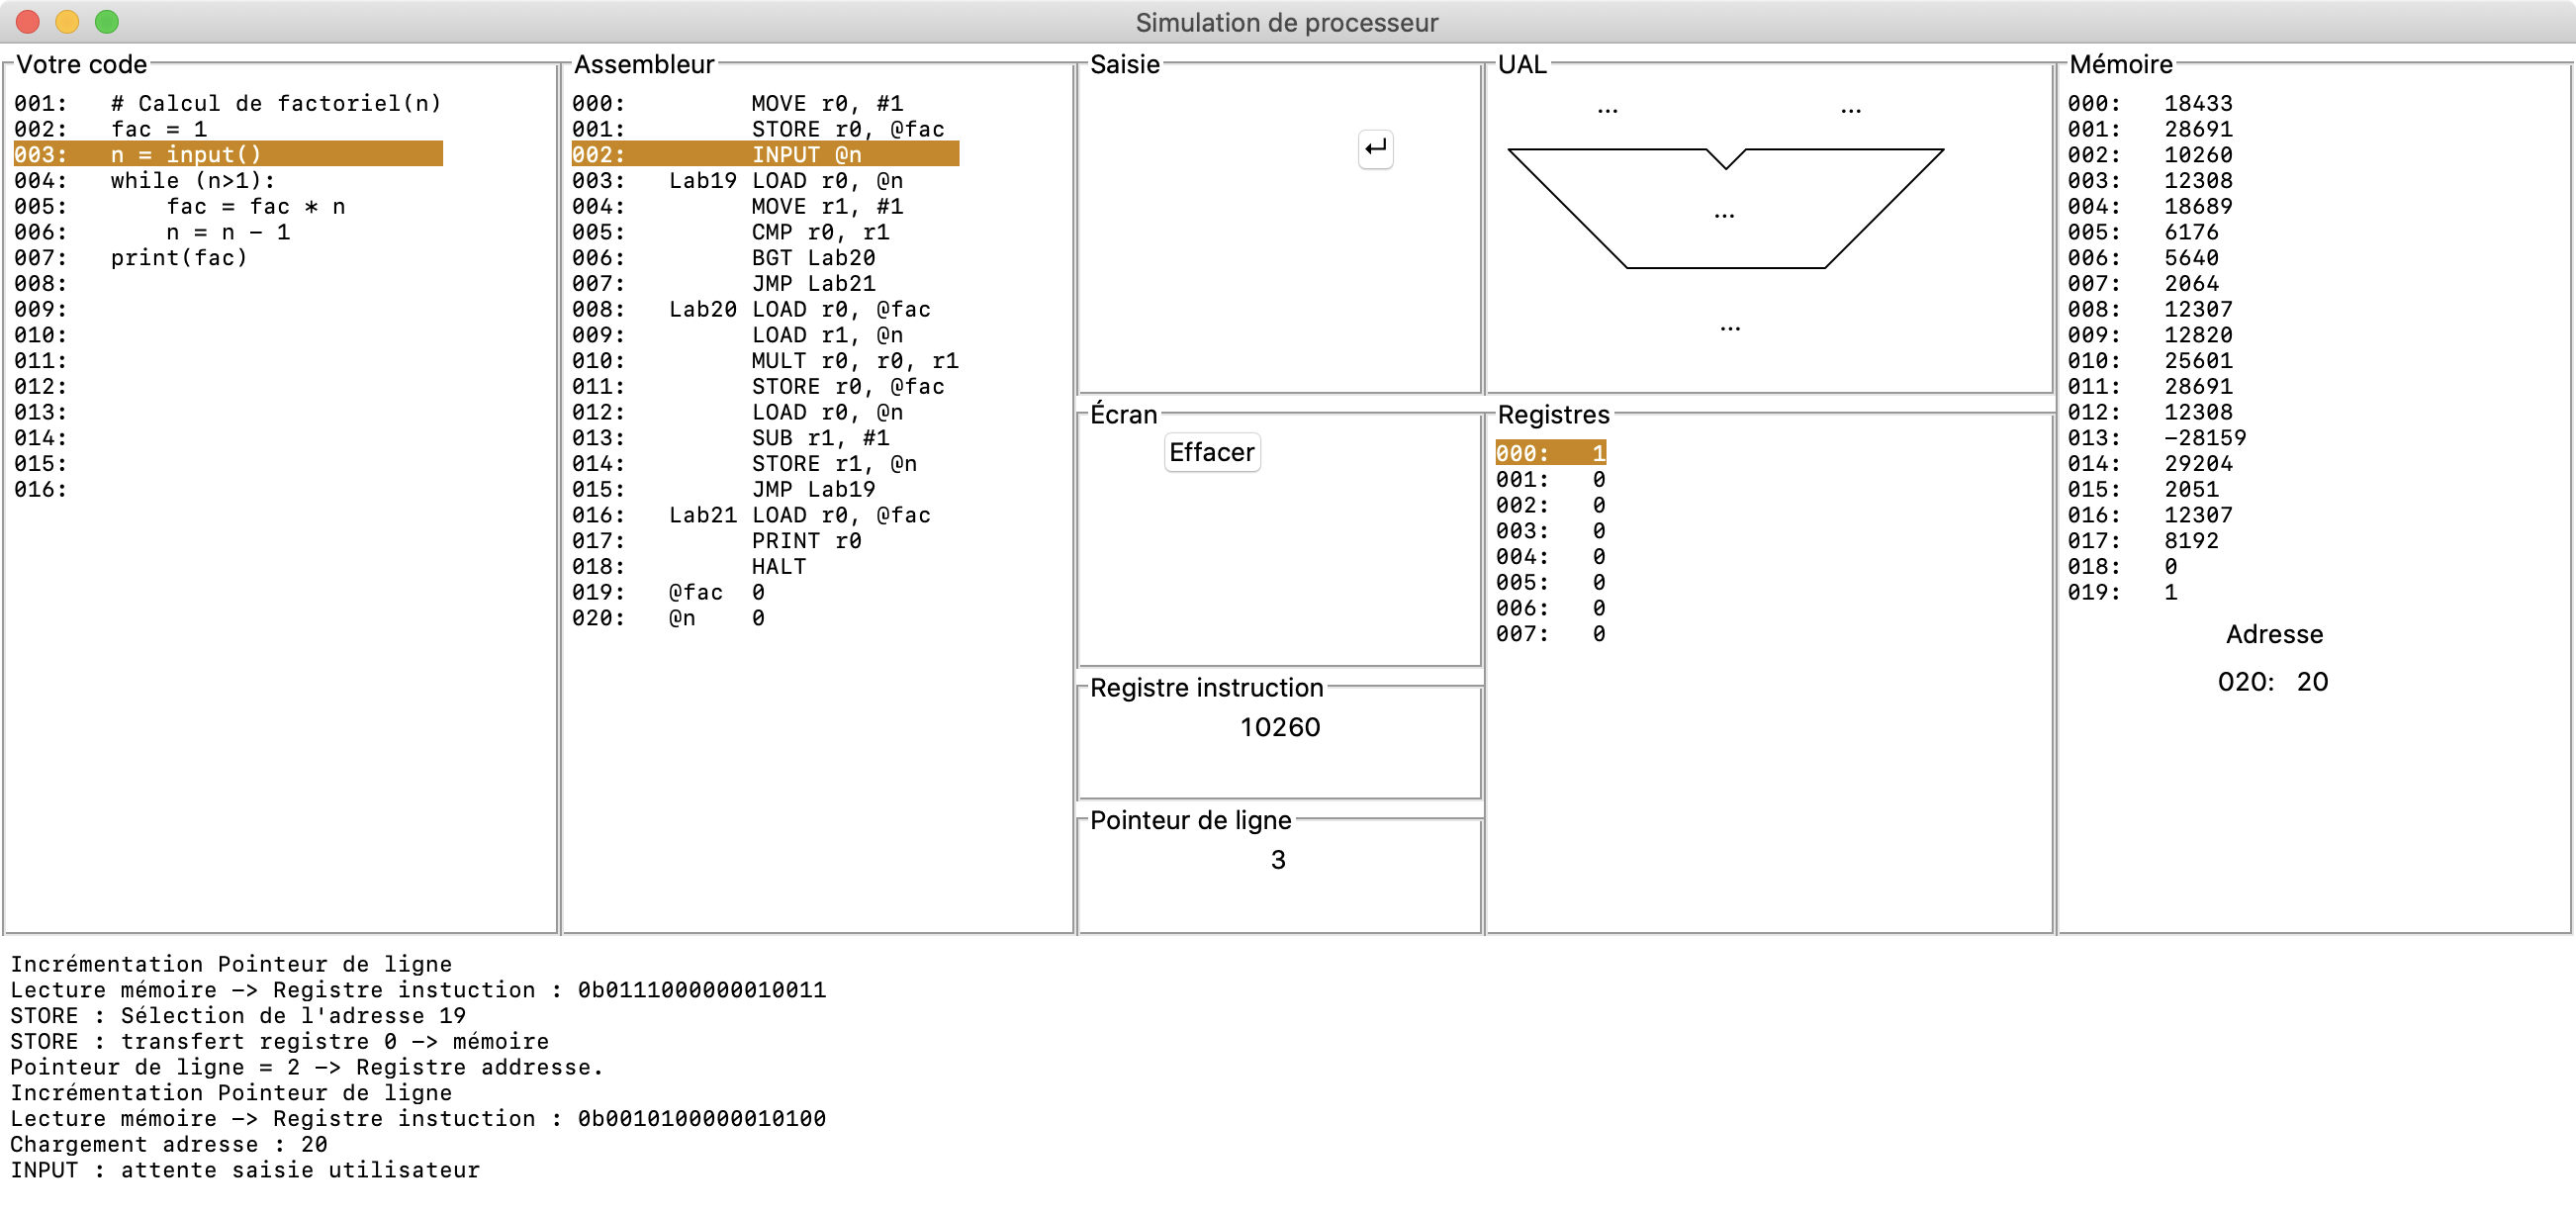
\includegraphics[height=8cm]{./Pictures/ExecGUI.png}
	\caption{Module Exécution}
\end{subfigure}
\caption{Interface graphique}
\end{figure}